\section{Použité technologie, frameworky a knihovny}
\label{sec-frameworks}

Výsledná aplikace byla implementována v jazyce {\bf C/C++} a využívá knihovnu {\bf OpenGL} \cite{openGL}. Ta poskytuje efektivní aparát pro práci s grafickým hardware a umožňuje využít většiny jeho nejnovějších vlastností a funkcí. Její výhodou je platformová nezávislost. Stejný kód by tedy mělo být možné přeložit jak pro Windows, tak pro systémy Unixového typu. Následně bylo využito několika dalších knihoven zjednodušujících práci se základní OpenGL:
\begin{description}
\item[GLFW] \cite{GLFW} sada knihovních funkcí určených pro snadné vytváření oken, OpenGL kontextů a mapování vstupních zařízení. Zachovává platformní nezávislost a uplatňuje se zejména ve fázi inicializace aplikace. Pomocí této knihovny je vytvořeno okno potřebných vlastností (podporuje i multisampling).
\item[GLUT] \cite{GLUT} sada nástrojů pro efektivnější práci. Obsahuje funkce pro vytváření oken a kontextů, mapování vstupů i pro práci s grafickými prvky.
\item[GLEW] \cite{GLEW} knihovna pro práci s rozšířeními (extenzemi) OpenGL. Zahrnuje zejména funkce pro zjišťování, zda ovladač grafického hardware danou extenzi podporuje.
\end{description}
Další knihovnou, která byla využita, je {\bf LODEpng} \cite{LODEpng}. Jde o jednoduchý dekodér a enkodér obrazového formátu PNG, který je distribuován formou jednoho \emph{.cpp} a jednoho {.h} souboru. Je s výhodou využit pro načítání obrázků do textur.

% obrázky zákl. ovládacích prvků
\begin{figure}[!hbt]
\begin{center}
$\begin{array}{cc}
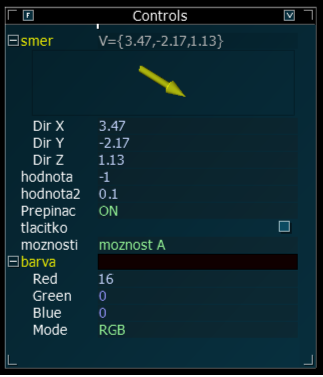
\includegraphics[width=0.35\textwidth]{./figures/ATWgui.png}&
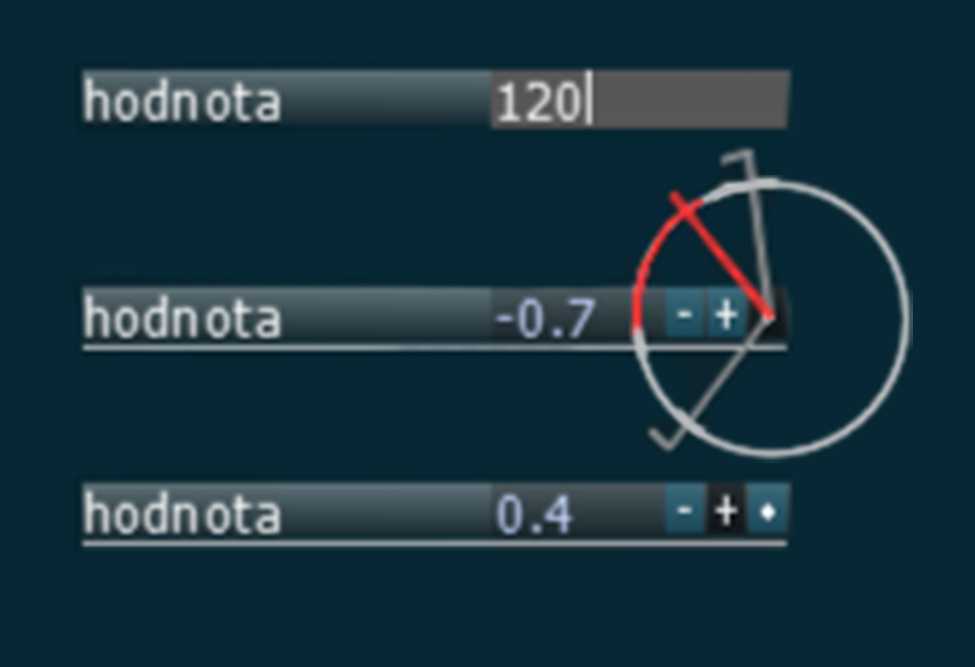
\includegraphics[width=0.3\textwidth]{./figures/ATWgui3.png}\\
(a)&(b)\\
\end{array}$
\caption[AntTweakBar, jednoduché GUI]%
{AntTweakBar, (a) ukázka základních ovládacích prvků (shora): ovladač směru, celočíselná skalární hodnota, desetinná skalární hodnota, dvoustavový přepínač, tlačítko, seznam možností, výběr barvy.  (b) různé způsoby zadávání hodnot (shora): přímé zadání, zadání pomocí tzv. RotoSlideru, pomocí krokovacích tlačítek \label{fig:ATWgui}
}
\end{center}
\end{figure}
Pro snadnou tvorbu grafického uživatelského rozhraní (dále jen GUI) byla využita knihovna {\bf AntTweakBar} \cite{AntTweakBar}. Ta umožňuje jednoduchou tvorbu grafických ovládacích prvků, které se nejčastěji používají při práci s 3D grafickou aplikací (viz obr. \ref{fig:ATWgui}). Těmito ovládacími prvky pak lze snadno bezprostředně a přímo ovlivňovat chování zobrazované scény - v tomto případě stromů.





